%%%%%%%%%%%%%%%%%%%%%%%%%%%%%%%%%%%%%%%%%%

\chapter{Ramsey method demonstration in prototype precession cell}\label{chap:lanl_ramsey_demonstration}

%%%%%%%%%%%%%%%%%%%%%%%%%%%%%%%%%%%%%%%%%%


%%%%%%%%%%%%%%%%%%%%%%%%%%%%%%%%%%%%%%%%%%%%%%

\section{Description of experimental setup (2017)}

%%%%%%%%%%%%%%%%%%%%%%%%%%%%%%%%%%%%%%%%%%%%%%


\begin{figure}
\centering
\begin{minipage}{.5\textwidth}
    \centering
    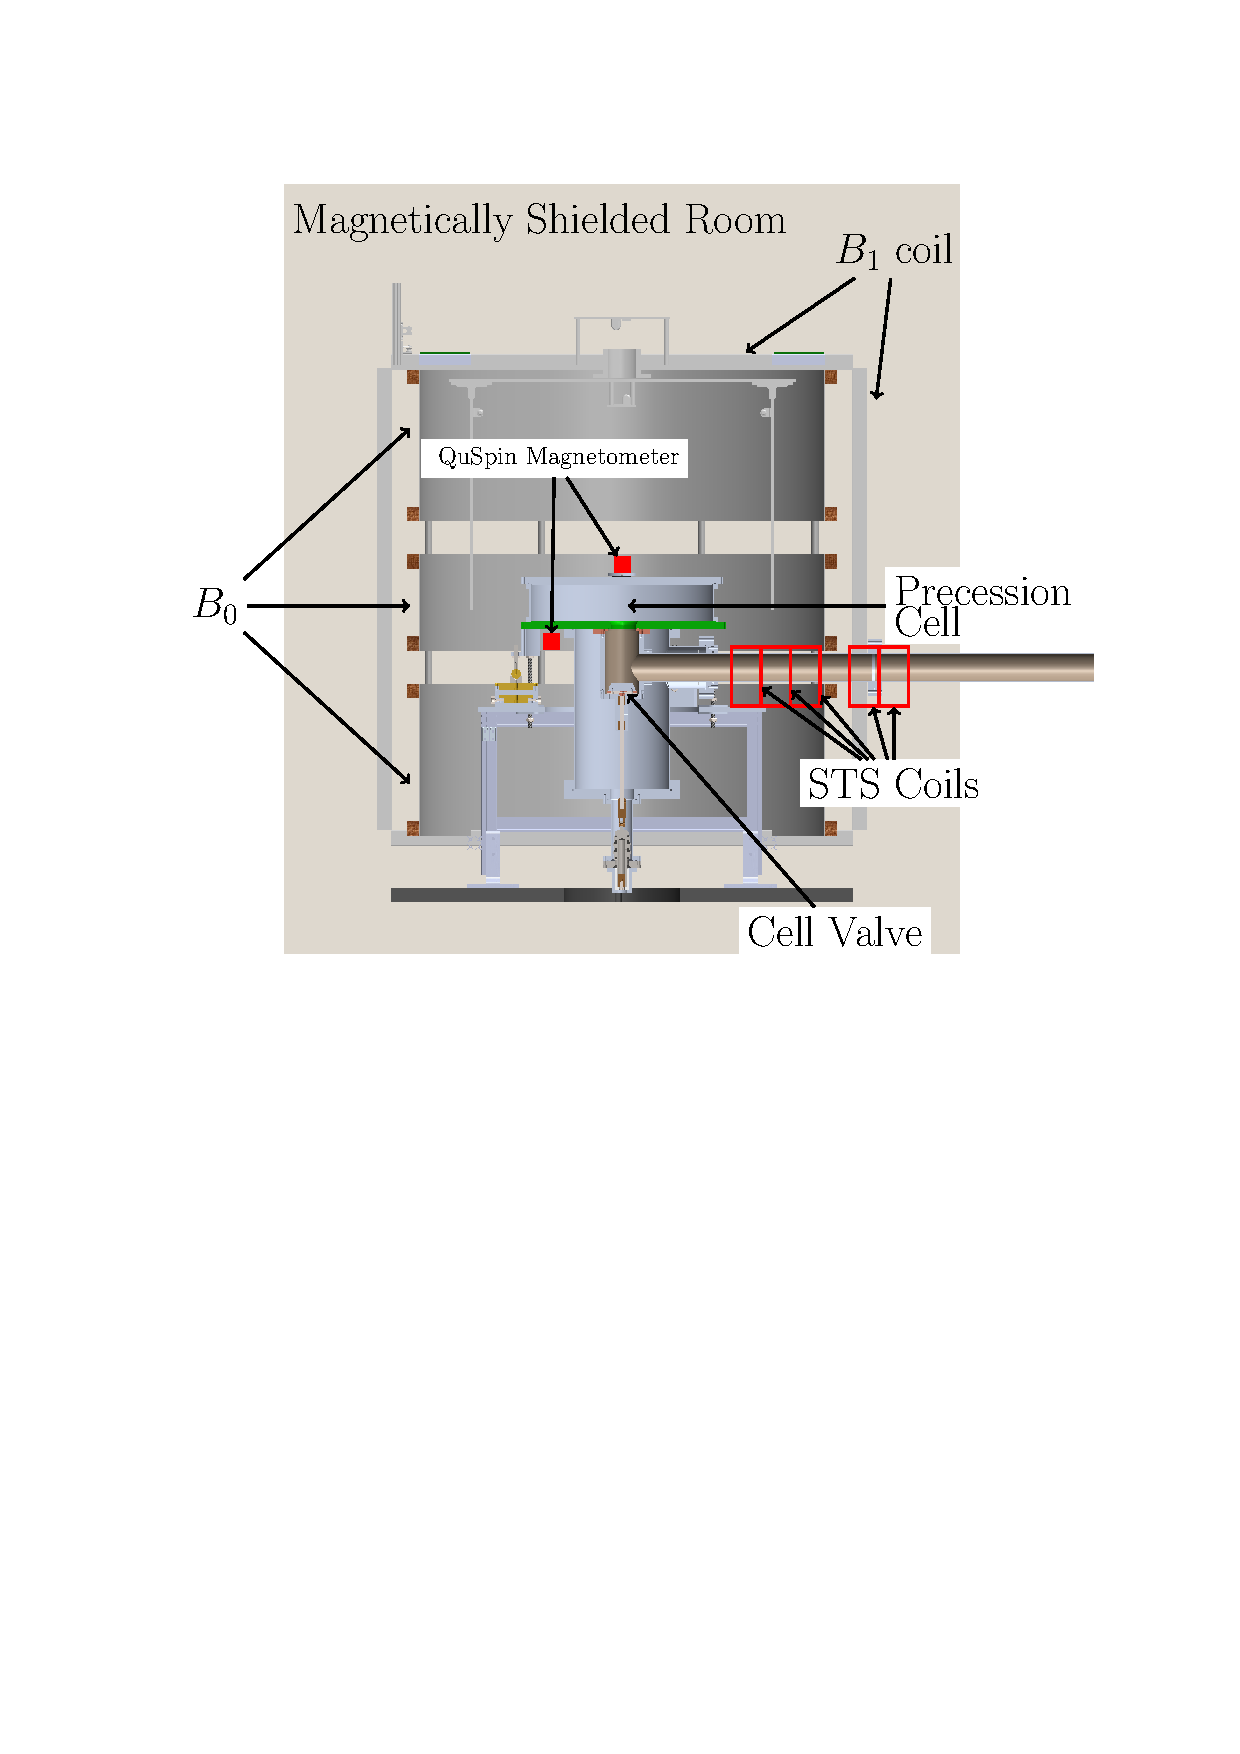
\includegraphics[width=\textwidth]{figures/ramsey2017_apparatus.pdf}
    \caption
    [Prototype experimental apparatus for measurements performed in 2017.]
    {Prototype experimental apparatus for measurements performed in 2017. Figure courtesy of Takeyasu Ito.}
    \label{fig:ramsey_2017_apparatus}
\end{minipage}%
\begin{minipage}{.5\textwidth}
    \centering
    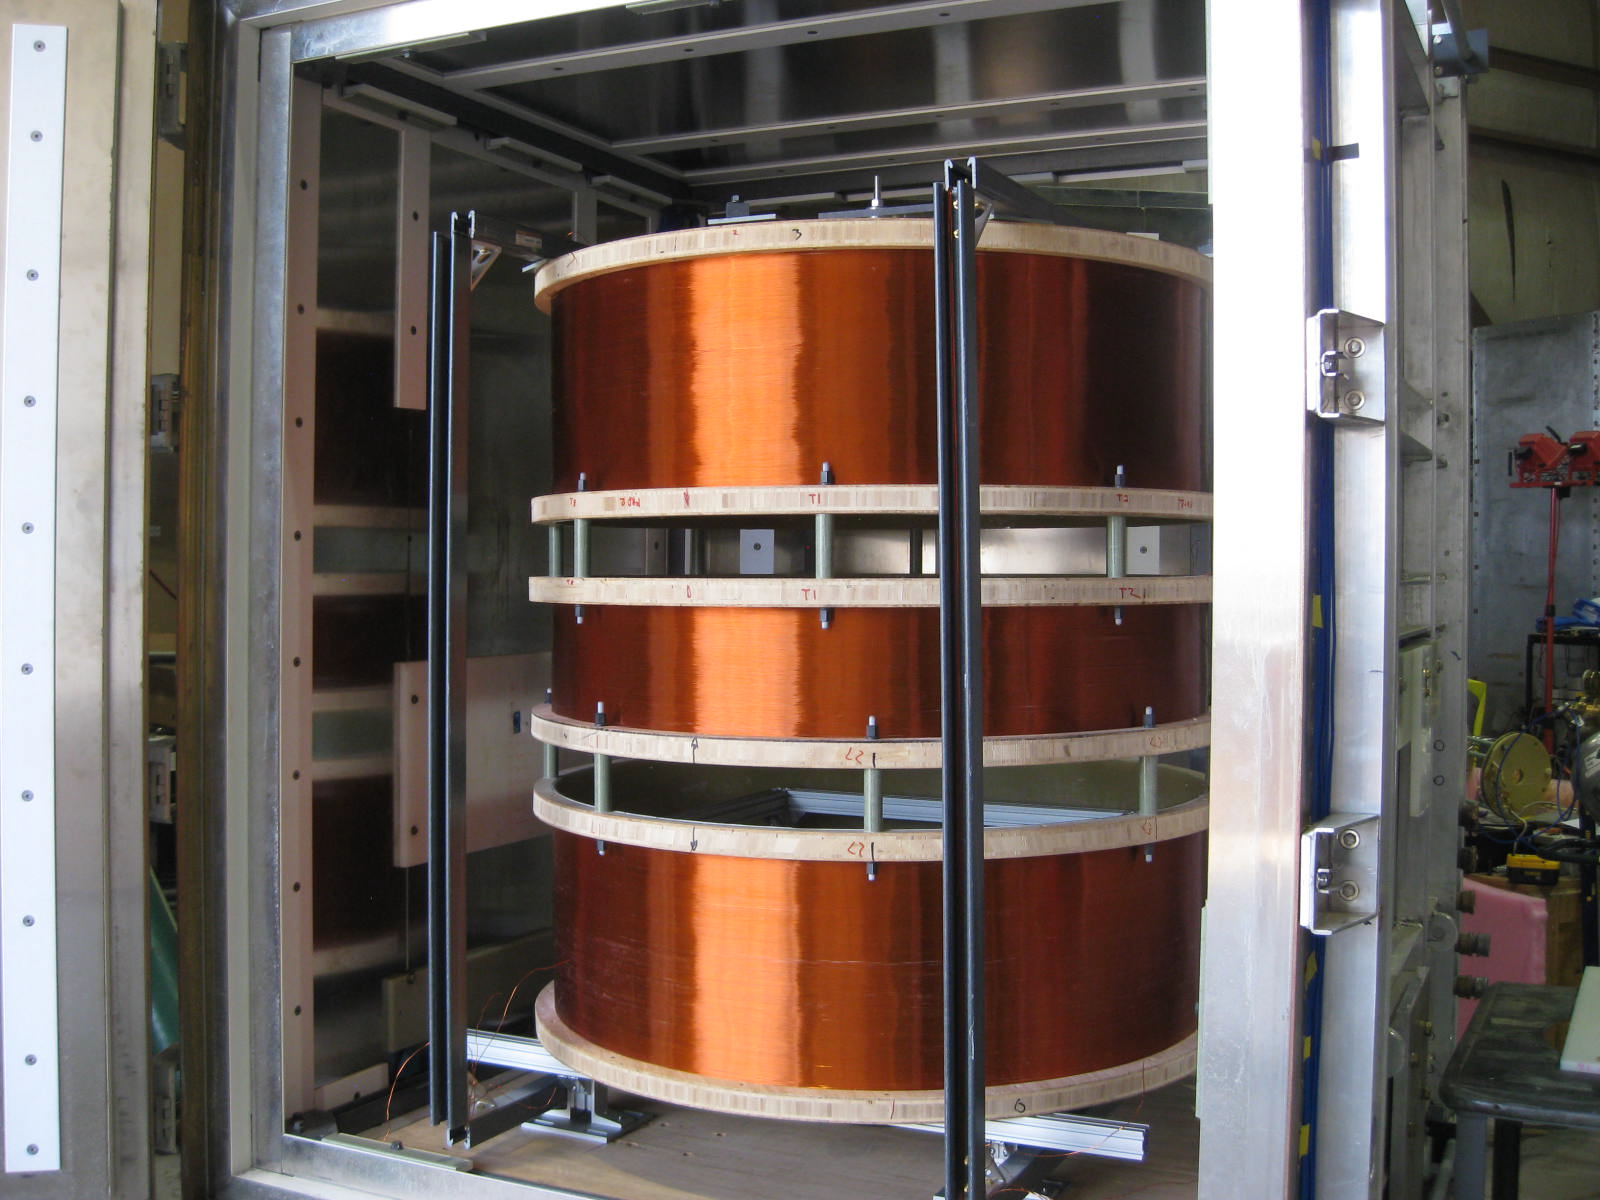
\includegraphics[width=0.8\textwidth]{figures/ramsey2017_B0_coil.png}
    \caption
    {$B_0$ coil prototype}
    \label{fig:ramsey_2017_B0_coil_prototype}
\end{minipage}
\end{figure}

Measurements took place in 2017. At the time, beamline configuration was slightly different. Aluminum window at the time was \qty{50.8}{\micro\meter} aluminum 5052. Rotary switcher. Valvebox was the same design as previous chapter. Additional solenoids along the beamline axis for transport up to the MSR

dPS wall storage chamber, NiP coating. Same spin analyzer configuration

Double layer MSR reduced ambient magnetic field to $\leq \qty{50}{nT}$. magnetometers were QuSpin total field magnetometers (now both are repurposed for magnetic impurity scanning). Quspins installed above and below

%%%%%%%%%%%%%%%%%%%%%%%%%%%%%%%%%%%%%%%%%%%%%%

\subsection
{
    \texorpdfstring{$B_0$ and transport coils}
                    {B0 and transport coils}
}

%%%%%%%%%%%%%%%%%%%%%%%%%%%%%%%%%%%%%%%%%%%%%%

\begin{figure}
    \centering
    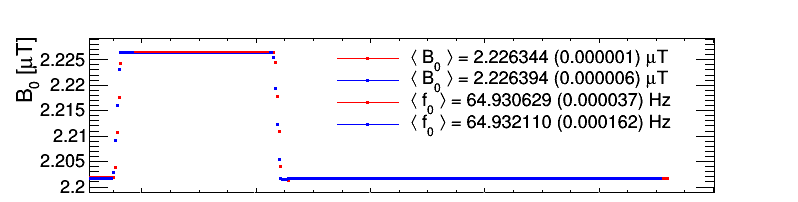
\includegraphics[width=0.8\textwidth]{figures/ramsey2017_B0.png}
    \caption
    [$|B_0|$ measured by the magnetometer located above the precession cell.]
    {$|B_0|$ measured by the magnetometer located above the precession cell. Blue and red lines refer to the measurement pair illustrated in Fig.~\ref{subfig:ramsey2017_t1_doublet}. The field drift between the two measurement periods was $\Delta B_0\approx\qty{50}{pT}$. When the STS transport coils were on during the fill and cell dump periods, $B_0\approx\qty{2.02}{\micro T}$.  During the measurement periods, $B_0\approx\qty{2.226}{\micro T}$. Figure courtesy of Robert Pattie Jr.}
    \label{fig:ramsey_2017_b0_map}
\end{figure}

Early prototype of the segmented solenoid, consisting of wire. 18AWG gauge, solid core copper, enamel-coated
magnet wire was wound on fiberglass-reinforced plastic frames. Design was based on \cite{gosling_gapped_solenoid_1974}. 

Opposite wound coils around B0 at top and bottom used for shimming. When cell valve closed, both magnetometers read the same value (within power supply resolution). Because this $B_0$ prototype was not sufficiently coupled to the MSR for flux return, there was a field 0 prior to entry, necessitating transport coils. The Segmented Tapered Solenoid (STS) tapered the magnetic field along the guide axis. Turned off after filling. See Fig.~ramsey2017-B0 to see impact of STS. \qty{2.226}{\micro T} during holding period


%%%%%%%%%%%%%%%%%%%%%%%%%%%%%%%%%%%%%%%%%%%%%%

\section
{
    \texorpdfstring{$T_1$ relaxation time measurement}
                    {T1 relaxation time measurement}
}

%%%%%%%%%%%%%%%%%%%%%%%%%%%%%%%%%%%%%%%%%%%%%%


\begin{figure}
\centering
%subfigure width gets "multiplied" by includegraphics width
\begin{subfigure}{.5\textwidth} 
  \centering
  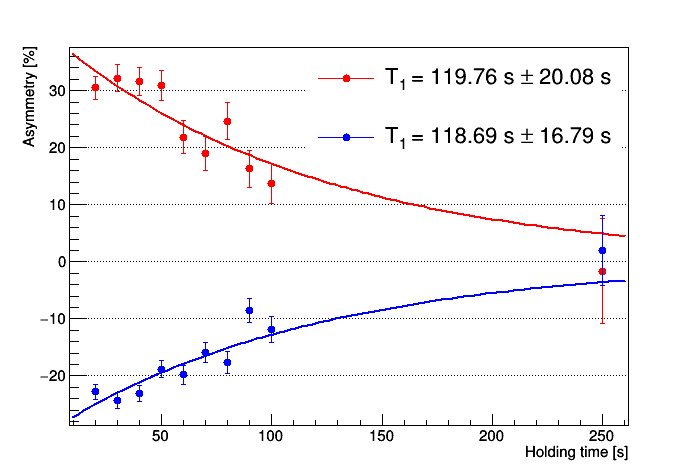
\includegraphics[width=\textwidth]{figures/ramsey2017_t1.png}
  \vspace{8pt}
  \caption{}\label{subfig:ramsey2017_t1_asymmetry}
\end{subfigure}%DO NOT REMOVE THIS '%'
\begin{subfigure}{.5\textwidth}
  \centering
  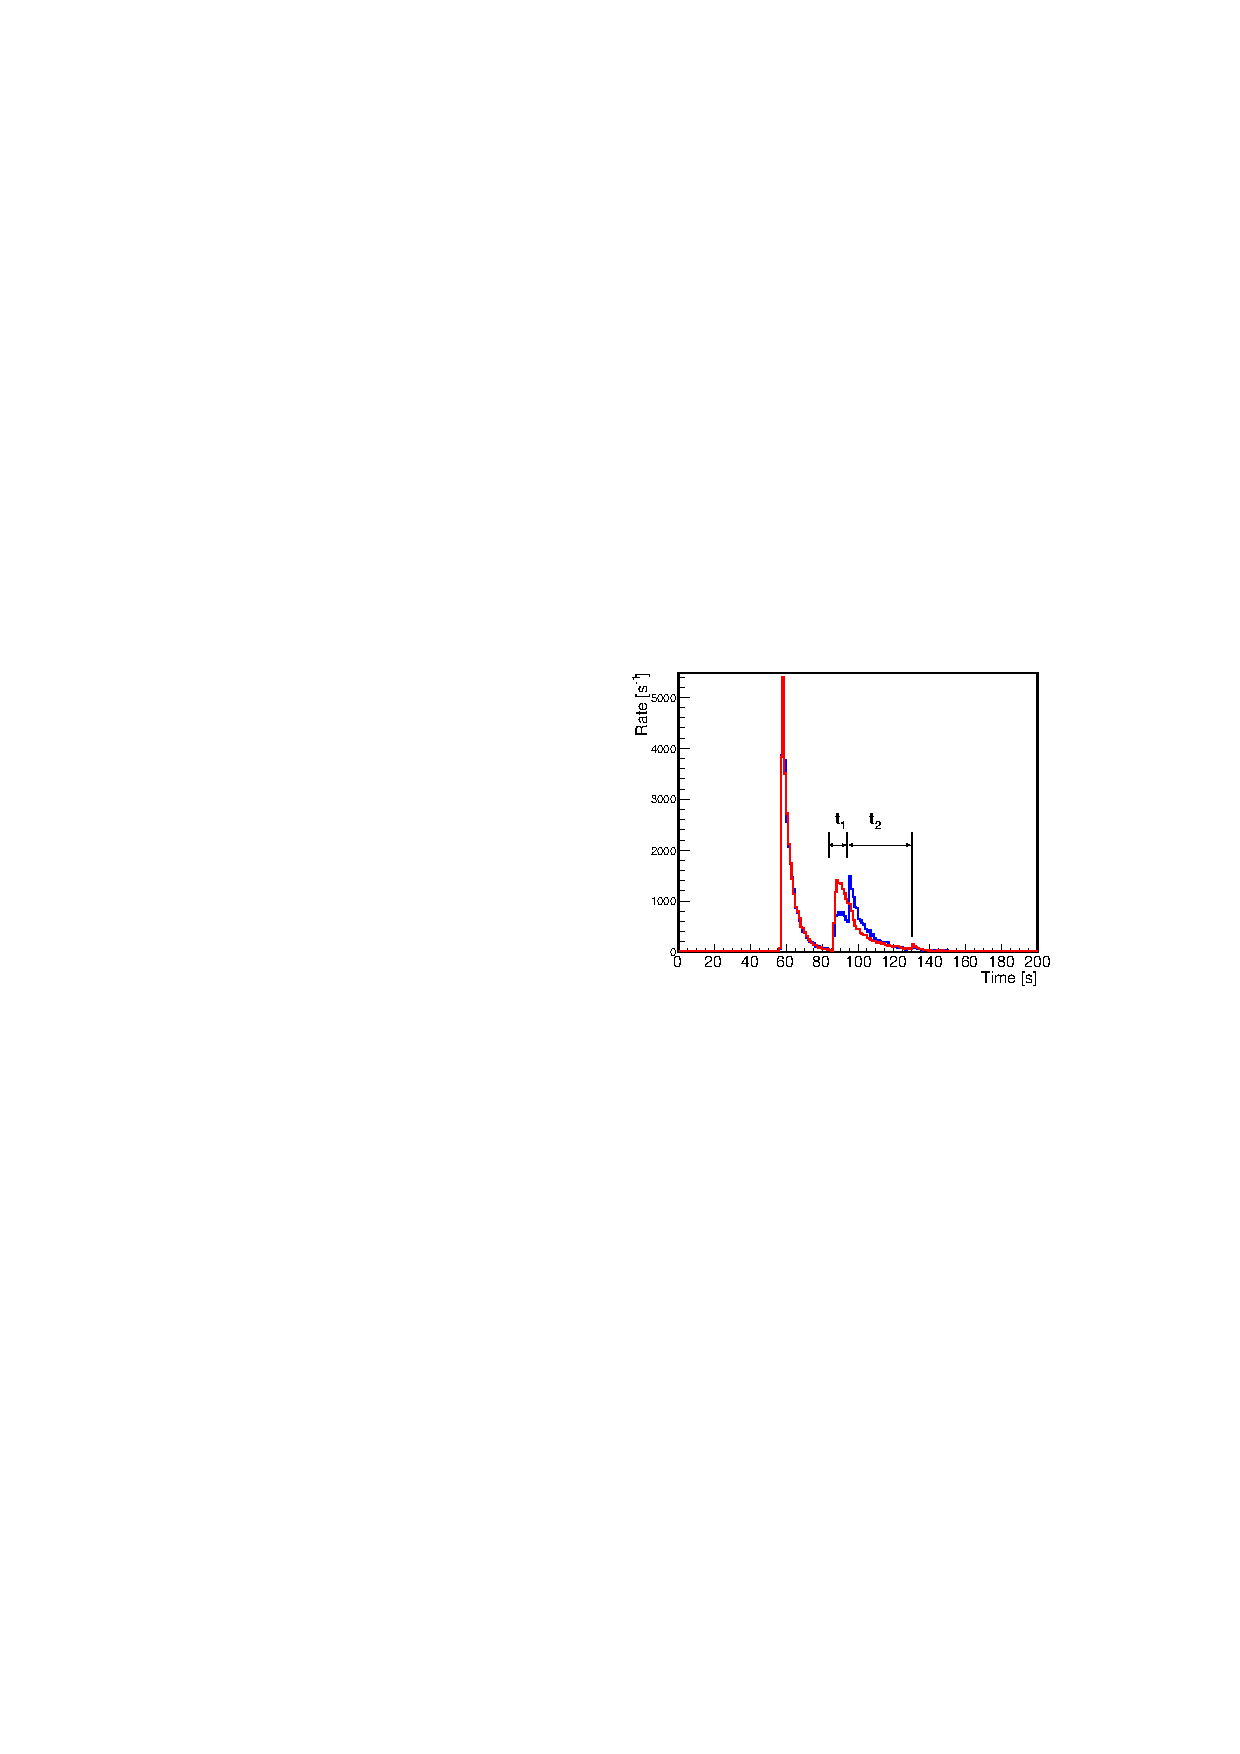
\includegraphics[width=\textwidth]{figures/ramsey_2017_t1_measurement_pair.pdf}
  \caption{}\label{subfig:ramsey2017_t1_doublet}
\end{subfigure}
\caption
    [Spin asymmetry as a function of holding time in the prototype apparatus.]
    {\textbf{(\subref{subfig:ramsey2017_t1_asymmetry})} Spin asymmetry as a function of holding time in the prototype apparatus. The red line refers to asymmetry during counting period $t_1$, and the blue line refers to asymmetry measured during counting period $t_2$. A fit of the measurements with a decaying exponential gives longitudinal spin relaxation time $T_1$. \textbf{(\subref{subfig:ramsey2017_t1_doublet})} Fill and dump sequences and counting periods. The red line refers to the sequence with the spin flipper toggling off-on-off during the cell dump, and blue refers to a on-off-on sequence. Figures by Robert Pattie Jr.}
\label{fig:ramsey_2017_t1}
\end{figure}

$T_1$ formulation from Sec.~\ref{sec:spin_relaxation}, Eq.~(\ref{eq:T1_dBdZ_mcgregor}). Fill and dump sequence following the methodology in Sec.~\ref{subsec:holdingTimeMeasurement} (as depicted in Fig.~\ref{fig:timeSpectrum}). 45 second preload period, 5 second filling. Short fill time used to limit depolarization time for UCN in the guide system. After storage the UCN were directed into the spin analyzer. Two measurements taken sequentially, a run pair Spin flipper off (on) 10 seconds, on (off) for 35, off (on) for 20. Refer to ramsey-2017-t1-measurement-pair

Assymetry is defined as
%
\begin{gather}
    A_i=\frac{\Gamma_{\text{on, }i}-\Gamma_{\text{off, }i}}{\Gamma_{\text{on, }i}+\Gamma_{\text{off, }i}}
    \label{eq:spin_asymmetry} 
\end{gather}
%
Counts in the detector normalized using the North beamline monitor (Fig.~\ref{fig:NorthBeamlineLayout}) as per Sec.~\ref{subsec:dataProcessing}. Should be noted that no leaks were observed in the data from these runs.  For holding times $<\qty{40}{s}$ a fit to the guide dump was required.

Assymetry shown in Fig.~ramsey2017-t1. Fitting a single exponential. Mean time $\langle T_1 \rangle=\qty{199(13)}{s}$. Assymmetry at $t=0$ is 0.3, which is worse than a flow through measurement (Fig.~\ref{fig:spin_flipper_efficiency}). Swapping dPS walls with NiP did not change $T_1$, suggesting relaxation time influenced most by gradients.

Use Eq.~(\ref{eq:T1_dBdZ_mcgregor}). Estimate mean wall collision time $\tau_\text{c}=4V/(vA)=\qty{36.7}{ms}$ (Appx.~\ref{appx:ucn_effusion}). Gives $\partial B_0/\partial z\approx \qty{12}{\micro G\per cm}$ in the chamber. At the time had no in situ measurement method available to confirm gradient.

%%%%%%%%%%%%%%%%%%%%%%%%%%%%%%%%%%%%%%%%%%%%%%

\section{Rabi measurement}

%%%%%%%%%%%%%%%%%%%%%%%%%%%%%%%%%%%%%%%%%%%%%%

\begin{figure}
    \centering
    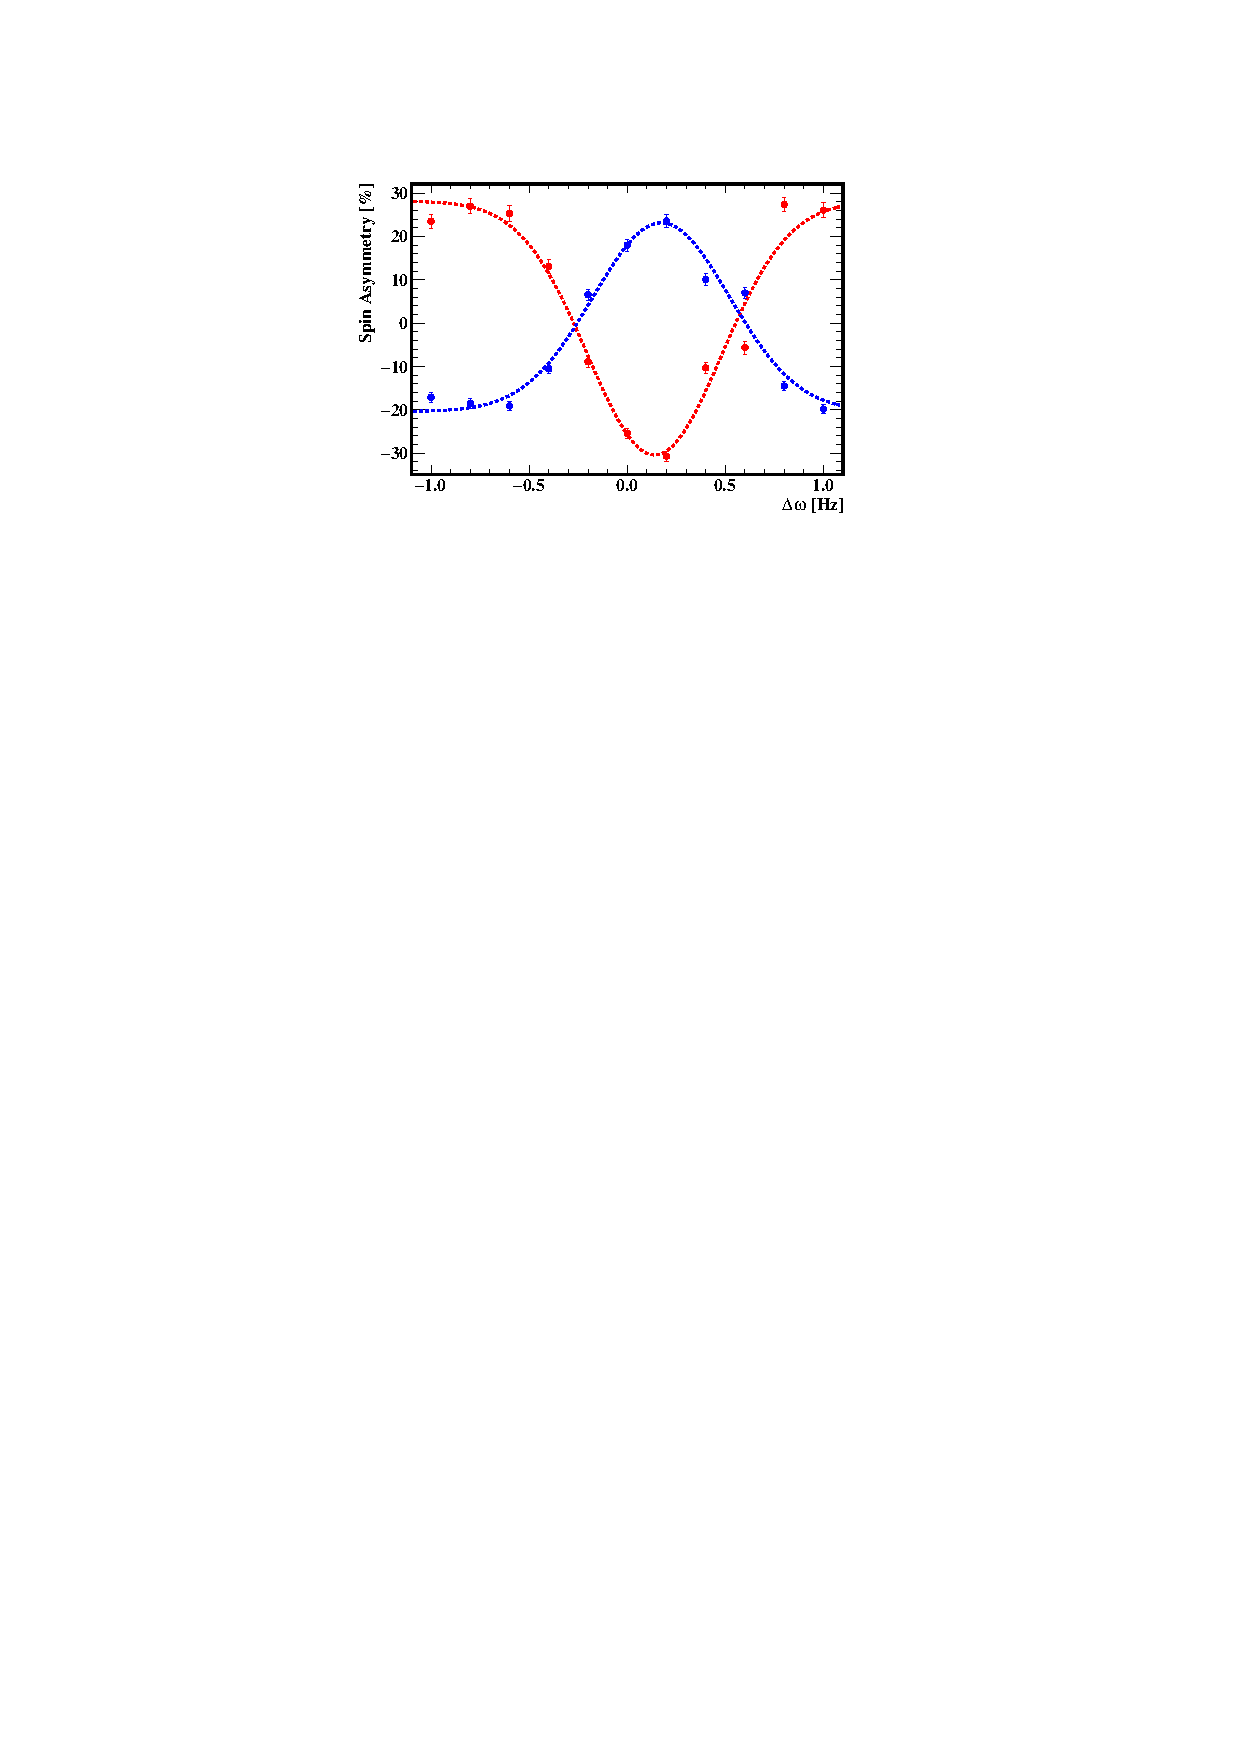
\includegraphics[width=0.55\textwidth]{figures/2017_rabi_fringe.pdf}
    \caption
    [Rabi fringe measured in the prototype apparatus.]
    {Rabi fringe measured in the prototype apparatus. A plot of spin asymmetry (\ref{eq:spin_asymmetry}) as a function of $\pi$ pulse frequency. Figure by Robert Pattie Jr.}
    \label{fig:rabi_fringe_2017}
\end{figure}

30 second total holding time. 5 seconds after the start of the holding period a 1 second $\pi$ pulse was applied. Frequency range applied was $\qty{64.5}{Hz} \pm \qty{1}{Hz}$ in step sizes \qty{0.2}{Hz}

%%%%%%%%%%%%%%%%%%%%%%%%%%%%%%%%%%%%%%%%%%%%%%

\section{Ramsey measurement}

%%%%%%%%%%%%%%%%%%%%%%%%%%%%%%%%%%%%%%%%%%%%%%

\begin{figure}
    \centering
    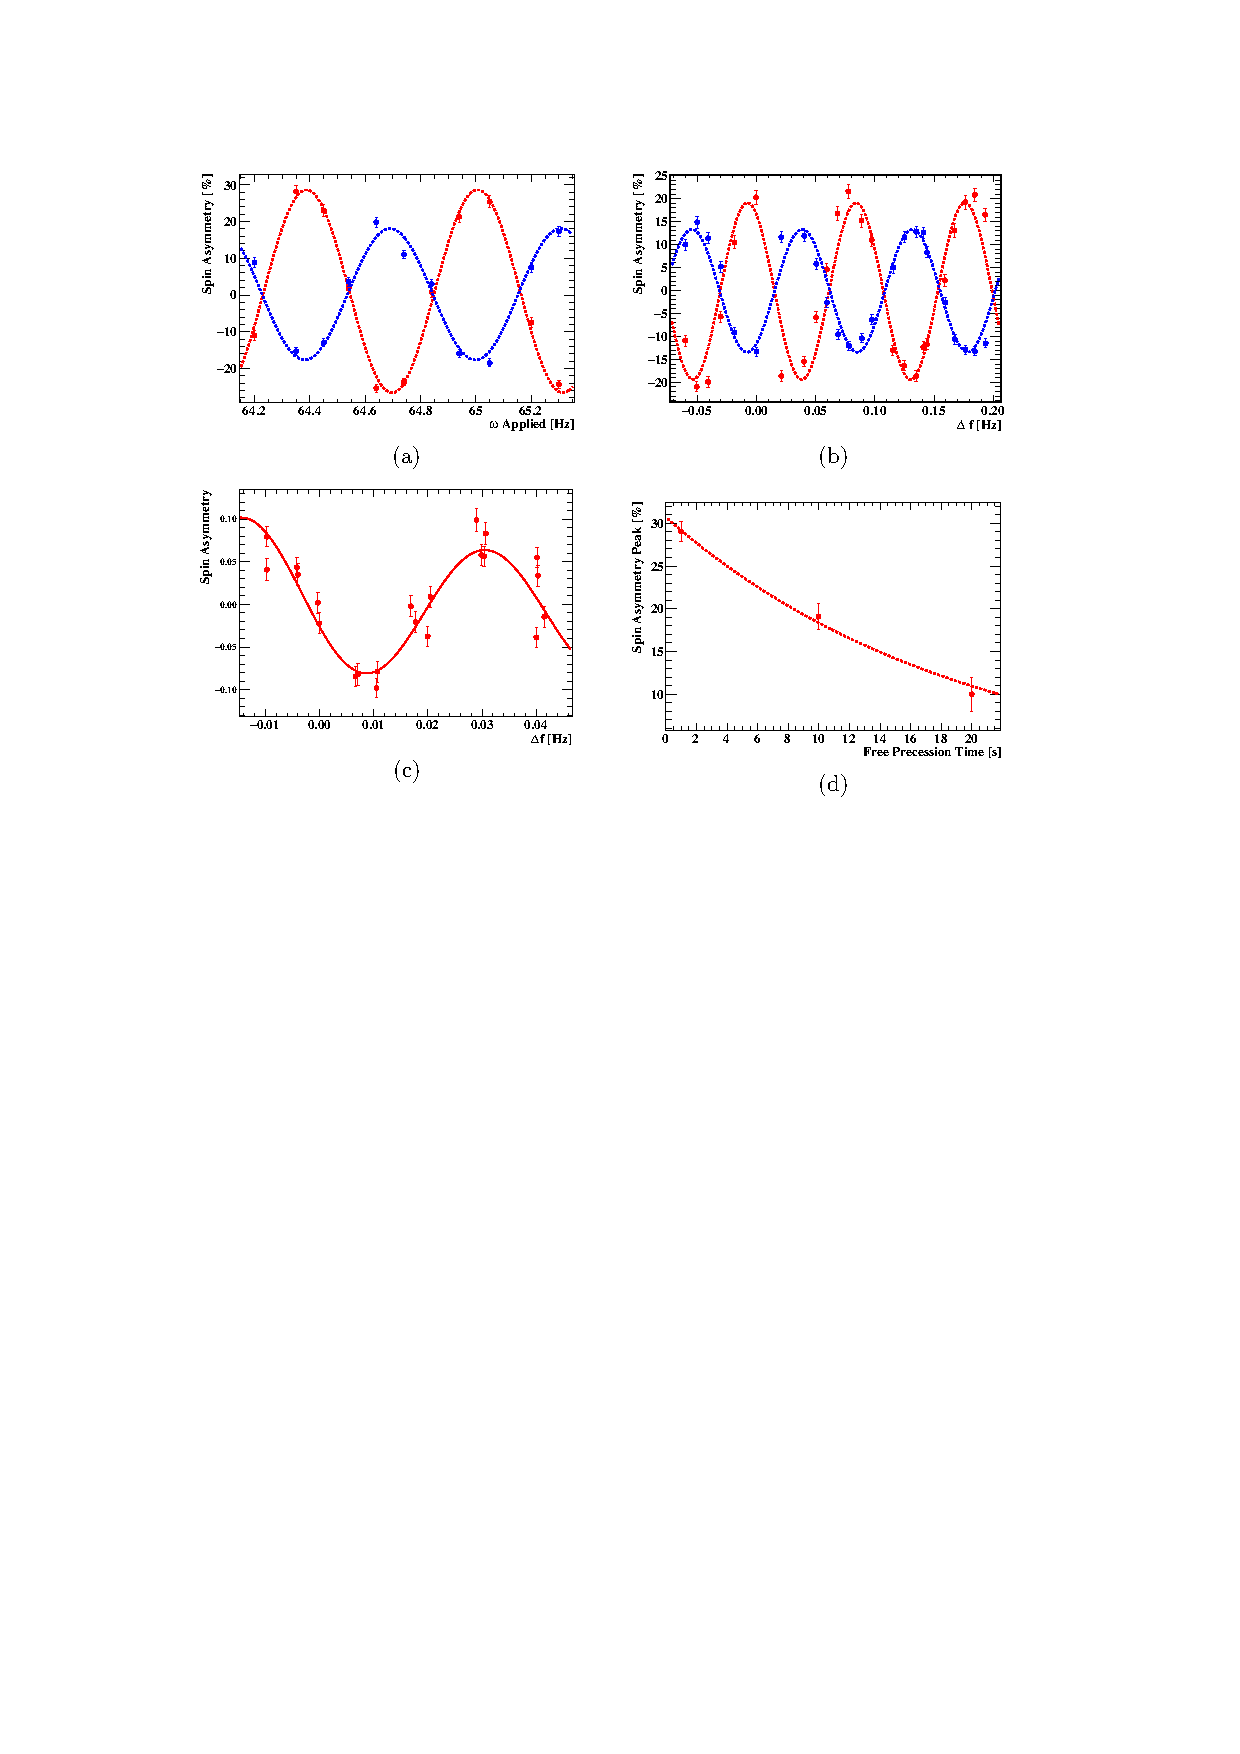
\includegraphics[width=\textwidth]{figures/2017_ramsey_fringes.pdf}
    \caption
    [Ramsey fringes measured in the prototype apparatus.]
    {Ramsey fringes measured in the prototype apparatus. Free precession period $\gls*{T_fp}=\text{\textbf{(a)} }\qty{1}{s}$, \text{\textbf{ (b)} }$\qty{10}{s}$, \text{\textbf{ (c)} }$\qty{20}{s}$. Panel \textbf{(d)} shows a fit of spin asymmetry (\ref{eq:spin_asymmetry}) as a function of \gls*{T_fp}. A fit of \textbf{(d)} with a decaying exponential gives $T_2=\qty{19.5(2.7)}{s}$. Figures provided by Robert Pattie Jr. and Takeyasu Ito.}
    \label{fig:ramsey_fringes_2017}
\end{figure}

Similar to Rabi sequence, $\pi/2$ pulse 0.5 seconds each. Three different precession times measured. Total holding time still 30s

Polarization decreased as free precession increased. Summarize panel (d). For each free precession period, the max polarization decreased. Fit to a decaying exponential gives transverse relaxation time $T_2=\qty{19.5(2.7)}{s}$ (because spins are precessing in x--y). See Eq.~(\ref{eq:T2_mcgregor}). To determine diffusion constant (\ref{eq:ucn_diffusion_constant}) Assume \ucn diffusivity $\sim 10\%$ gives $D_\text{ucn}\approx \qty{2.2}{m^2 \per s}$\cite{golubUCN}. Estimate of gradient, assuming x and y contributions about the same, gives $\partial B_z/\partial r \approx \qty{18}{\micro G \per cm}$ 

%%%%%%%%%%%%%%%%%%%%%%%%%%%%%%%%%%%%%%%%%%%%%%

\section{Pulse sequence instrumentation}

%%%%%%%%%%%%%%%%%%%%%%%%%%%%%%%%%%%%%%%%%%%%%%

Pulse sequence used SRS DS345 with amplitude modulated by a DG535 pulse generator. Refer to appendix \ref{appx:gpib_usb_pulse_sequence} for code.